\documentclass[11pt]{article}
\usepackage{framed, color}
\usepackage{textpos}
\usepackage{natbib}
\usepackage[top=1in, bottom=1in, left=.75in, right=.75in]{geometry}
\usepackage{color}
\usepackage{hyperref}
\usepackage{textcomp}
\usepackage{graphicx}
\usepackage{fancybox}
\usepackage{setspace}
\hypersetup{colorlinks=false, urlcolor=blue, citecolor=black}
\usepackage{soul}
\usepackage{geometry}
\usepackage{color}
\newgeometry{top=1in, bottom=1in, left=.75in, right=.75in}
\usepackage{fancyhdr}
\usepackage{wrapfig}
\usepackage{mdframed}
\pagenumbering{arabic}
\usepackage{fontspec}
\setmainfont{Arial}

\linespread{1.1}

\begin{document}


%\parindent 0.000000001in
\setlength{\parindent}{1cm}
\setcounter{page}{0}
\pagenumbering{arabic}

\fancyhead[CO]{Matthew D. MacManes | Research Strategy}
\pagestyle{fancy}



%\noindent \large{\textbf{\textsc{A. Personnel:}}} \\
%\normalsize 
%
%\noindent \textsc{MacManes, Matthew D} \\
%Department of Molecular, Cellular \& Biomedical Sciences. \\
%University of New Hampshire, Durham, NH 03824 USA \\
%
%\noindent
%\noindent STATUS: PI (Beginning Investigator)\\
%TITLE: Assistant Professor \\
%ROLE: Dr. Matthew MacManes will be responsible for all aspects of the project including design, collection and analysis of next-generation sequencing data, genome and transcriptome assembly, analyses of differential gene expression across experimental manipulations, generation and analysis of physiology data, supervising undergraduate and graduate students, postdocs at the University of New Hampshire, writing manuscripts, presentation of results at scientific conferences, and public outreach in New Hampshire.
%\newpage

\setcounter{page}{1}
%\noindent \large{\textbf{\textsc{2. Project:}}}
\normalsize 
\begin{center}
\textsc{{i. Significance}} \\
\end{center}

Dehydration, whether caused by exposure to extreme environmental conditions, water deprivation, or by infection (e.g. diarrheal illnesses) represents a significant threat to human life. When death is avoided, dehydration may lead to chronic health conditions like renal failure. While the mechanisms underlying physiological compromise are well characterized [ref], some animals possess the ability, much unlike humans, to osmoregulate despite extreme heat and a complete lack of extrinsic water intake [ref]. Specifically, highly adapted desert mice may never drink water [ref], produce an extremely viscous urine (or no urine at all) [ref], and excrete urea in the form of uric acid crystals in the feces [ref]. Focusing on osmoregulation, patterns of renal gene expression have been shown to be highly derived in some desert adapted rodents (e.g. \textit{Dipodomys} [ref]), but not in others like (\textit{Notomys}), and therefore the extent to which differences in gene expression underlies phenotype remains unknown. In addition to its' generality, both studies of non-model organisms focus on a limited number of genes, and therefore may not appropriately assay the complexity of the genetics of extreme renal osmoregulation. In contrast with this work, several studies attempting to understand the effects of dehydration in model organisms (e.g. \textit{Mus} and \textit{Rattus}) exist, though while these works benefit from an extensive genomic and physiologic toolbox, that they lack the appropriate phenotype (extreme osmoregulatory abilities) limits insight. In summary, the study of extreme renal osmoregulation is hindered on one hand by a lack of tools, and on the other by a lack of an appropriate phenotype. This limitation may undercut our ability to efficiently develop novel therapies directed at mitigating the untoward effects of dehydration. \\

The proposed research uses a novel approach integrating physiology, evolutionary genomics, and computational biology to better understand how animals survive in what appear to be non-survivable conditions. I develop the genomic and physiologic tools in a novel model for the study of extreme osmoregulation, \textit{Peromyscus eremicus}. It's contribution is to effectively leverage the power of a sophisticated toolset of a model organism against a uniquely adapted rodent, which will allow for a synthetic understanding of extreme osmoregulation, and ultimately novel insights into the cause of - and cure for - dehydration related mortality and morbidity.
\normalsize 
\begin{center}
\textsc{{ii. Innovation}} \\
\end{center}

In spite of modern medicine, millions of people die from dehydration, and millions more are affected by chronic kidney disease. The proposed work recognizes that successful treatment requires an appropriate model, and while traditional models are powerful tools, they lack the biology (extreme osmoregulation) upon which a more successful phenotype may be modeled. The desert-adapted rodent \textit{P. eremicus} retains many of the beneficial characteristics of model organisms, while augmenting existing biomedical infrastructure. In addition to this fundamental innovation, the project it innovative in a number of other ways.
\begin{itemize}
\item Leverage an unprecedented level of control over the experimental environment by use of a desert chamber where natural conditions can be replicated while preserving the ability to manipulate water availability. 
\item Link detailed information on physiology and metabolism to genomic information using powerful and novel analytical tools under active development in the lab.

\end{itemize}

 

\newpage



\noindent \textbf{Aim 1:} \ul{Using captive desert-adapted mice, I will correlate multiple physiological variables, as well as their genomic underpinnings to differences in temperature, relative humidity, and water availability.} \\

\begin{wrapfigure}{r}[0pt]{0.5\textwidth}
\hypertarget{Figure 1}{}
\vspace{-5mm}
\begin{mdframed}
  \begin{center}
    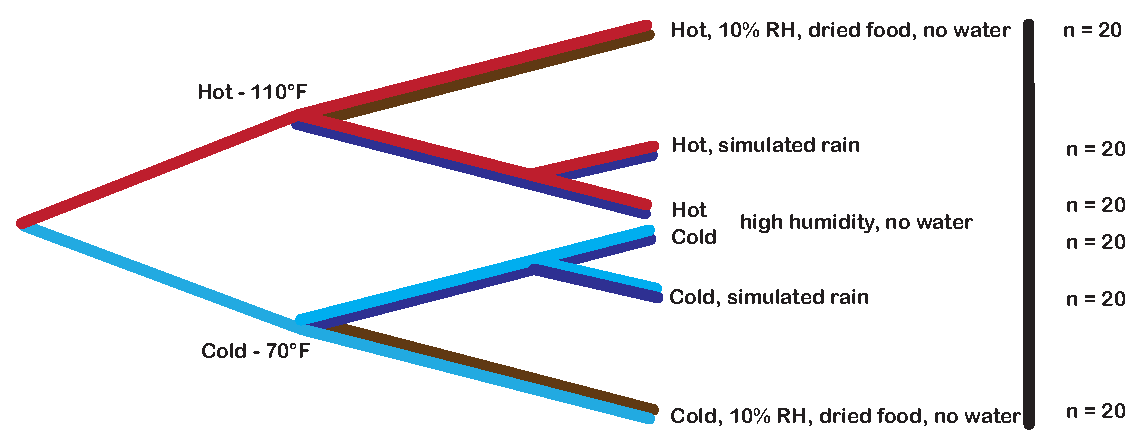
\includegraphics[width=1\textwidth]{exp_design_fig.eps}
  \end{center}
  \caption{\small{Animals are relegated into either hot or cold treatments. Within treatments (n=10 per treatment), animals are exposed to two weeks of varying levels of aridity, from simulated rainfall where water is available \textit{ad libitum}, to dry, where no water is available. RH=relative Humidity}}
\end{mdframed}
\end{wrapfigure}
To better understand the physiological effects of desert conditions on rodents, I will relate multiple physiological variables to differences in temperature, relative humidity, and water availability. These experiments (and those described under Aim 2) are fundamentally linked to a series of environmental manipulations, described in \hyperlink{Figure 1}{Figure 1}. I hypothesize that, as a result of unique mechanisms related to solute and water balance, that average electrolyte concentrations will remain relatively constant throughout various experimental manipulations, but the variance in measured levels between individuals will increase in the most extreme conditions. \\


\noindent \textbf{Aim 1a:} Define the relationship between temperature | humidity | water availability and physiological state. \\

From all animals in experimental treatment groups (n=10 * 6 treatments=60 animals), I will collect a urine sample, and measure specific gravity and urine osmolality using an Atago UG-$\alpha$ urine refractometer. Serum electrolytes including potassium, sodium, BUN, creatinine, calcium and bicarbonate ion concentration will be measured. Metabolic parameters including carbon dioxide production and oxygen consumption will be measured will be measured during a twelve hour period at the end of the experimental manipulation, just prior to euthanasia, using a standard metabolic chamber (Sable Inc.) modified for use in the desert chamber. \\


\noindent \textbf{Aim 1b:} Define patterns of gene expression | isoform use | methylation given differences environmental condition. \\

{I will understand the genetic response to extreme heat and aridity via a series of bisulfite sequencing and RNAseq experiments, and will link these patterns to individual physiologic state as defined in Aim 1.} Differences in renal methylation patterns and mRNA gene expression will be tested using the 10 individuals per treatment group (n=60 total, specified above). I hypothesize that genes responsible for water and solute transport will be particularly active in the most extreme conditions.  

For analysis of the bisulfite sequence data, an accurate genome assembly is required. Using the existing draft genome (sequenced using startup funds) as a starting point, I will complete the genome assembly of the primary study organism, \textit{Peromyscus eremicus}. This process will be significantly aided by leveraging the existing genome sequence data available from several other \textit{Peromyscus} species. Specifically, an additional 60X coverage Illumina dataset using 150bp paired end and mate-pair sequencing will supplement the current 40X dataset. Simultaneous with this, I will sequence up to 10X coverage using long-read PacBio sequencing. A short-read assembly of Illumina data will be done using AllPaths-LG \citep{Maccallum:2009du}.  Illumina contigs will be assembled with the corrected PacBio data using the software package SGA \citep{Simpson:2012ef} or an overlap-layout-consensus assembler (\textit{e.g.} Celera, \cite{Miller:2008jx}) to generate a primary \textit{de novo} genome assembly. Assemblies will be validated by use of the CEGMA \citep{Parra:2007df} and REAPR \citep{Hunt:2013hj} algorithms. In general, this approach has been shown to be successful in producing high quality draft assemblies, though multiple assembly methods will be evaluated as per the findings of my previous work \citep{Bradnam:2013gx}.

To annotate the genome, RNA and smRNA sequence data from several tissues, including liver, kidney, and brain will be generated. Sequence data will consist of Illumina strand-specific small-insert 150bp paired end sequencing. Each tissue type will be sequenced to a depth of 100 million reads.  Assembly will be accomplished using the Trinity software package \citep{Haas:2013jq,Grabherr:2011jb} after error correction \citep{MacManes:2013ec} and quality trimming \citep{MacManes:2013ex}. Annotation will be completed using the programs Trinotate (\url{http://trinotate.sourceforge.net/}) and Maker \citep{Cantarel:2008jo}. 

In addition to the assembly and annotation of the \textit{P. eremicus} genome, a secondary result of this work is methods development (\textbf{enhancing infrastructure}). To this end, I have already already released a transcriptome assembly pipeline (\url{http://sourceforge.net/projects/tamrs/}) and automated quality control software (\url{http://sourceforge.net/projects/qcpro/}). In addition to this, I am an active developer of the transcriptome assembly program Trinity and annotation software Trinotate. Given the popularity of high-throughput sequencing, the demand for these types of tool development programs will likely increase. \\


\noindent \textbf{Aim 1c:} Define the relationship between gene expression and physiology. \\















\newpage

\begin{center}
\textsc{{ii. Background}} \\
\end{center}

The study of adaptation, or the process through which animals become fitted to their environment has intrigued researchers for decades \citep{Darwin:1859tm, Fisher:1930wy}, though only recently have we had the ability to study the underlying genomic mechanisms. Interestingly, researchers interested in understanding the genetics of adaptation have the ability to ground modern studies of genetics on decades of work aimed at understanding the ecological context within which adaptation occurs. One particularly salient example of the connection between studies of ecology and natural history and modern genomics can be found in the study of physiologic adaptation to desert conditions. Here, remarkable physiologic, morphologic \citep{Dickinson:2007jn,Huntley:1984us,SchmidtNielsen:1950wg,SchmidtNielsen:1952wp} and behavioral \citep{NAGY:1994vd} adaptation has been studied in the context of desert ecology. These studies provide a rich context for the current work, which aims to define the relationship between physiology and genomics in rodents able to thrive in amongst the most harsh of conditions on Earth.  

Though classic research relating morphology (especially renal ultrastructure) and physiology to desert adaptation has been done, we know virtually nothing about how extreme heat and aridity may affect other core physiological and metabolic processes. For instance, the maintenance of normal serum electrolyte concentration is challenging in the context of desert conditions. Indeed, electrolyte derangement is often the ultimate cause dehydration-related death, yet for the vast majority of desert animals, we know nothing of electrolyte balance - not even typical values! Understanding these critical processes is fundamental to our understanding of physiological adaptation, and will be accomplished as part of this project. 

Lastly, the genomic processes related to desert survival have yet to be characterized. The few studies of genetics that have been done have focused on the role of single members of the Aquaporin gene family (but see \cite{Bartolo:2007hy}), which are large membrane-bound proteins that are critically involved in renal water transport \citep{Kwon:2009bv,Verkman:2002ww,Brown:1995vo,Nielsen:1995cb}. These studies have shown that changes in Aquaporin (AQP) protein abundance and expression may be related to water availability \citep{Boselt:2009fb, Gallardo:2005fm,Bozinovic:2003eg}. In addition to changes in expression, another study showed that the AQP4 pathway was completely lost in the desert rodent \textit{Dipodomys merriami merriami} \citep{Huang:2001ti}. Despite these studies, we have a limited understanding of the genomics of renal water and solute regulation in desert animals. While AQPs are functionally important, water and solute balance is extraordinarily complex, and therefore single-gene studies are necessarily limited in their purview. A more complete understanding of this phenotype and its mechanistic underpinnings will require a sophisticated genome-level approach, which will be the outcome of the proposed research. 


\textbf{Specific Aim 1:}   

\textbf{Specific Aim 2:}  

\textsc{{Preliminary Data:}} To date, I have generated a RNAseq dataset that consists of approximately 30M 150nt SE Illumina reads from the same 5 animals housed in the 'cold/simulated rain' treatment group from which I collected physiology data. 

\textbf{Specific Aim 3:} Given that desert adapted mice, capable of surviving without water are as neonates dependent on liquid intake, \ul{the study of the ontogeny of physiologic water conservation is extremely interesting and relevant to the current work.} This phenomenon will be explored using neonate mice in the treatments listed in Aim 1, and methods described in Aim 2. Five neonate mice will be culled per treatment at 3 different timepoints (immediately after birth, mid-lactation, 1 day after weaning). I hypothesize that patterns of gene expression and methylation will resemble those common in conditions where water is available \textit{ab lib}.  
\begin{center}
\textsc{{iv. Broad Impacts}} \\
\end{center}
How desert animals survive without water is an intrinsically interesting example of extreme physiology and adaptation. Indeed, telling people of the remarkable story of a rodent that may never drink water is immediately captivating. Having told hundreds of people, including children, adults, scientifically literate and not, the most common response is something like "Wow! That is amazing. How do they do that?" I intend to \textbf{broaden dissemination} by capitalizing on this common response, using traditional and non-traditional methods. While lecture has been the mainstay of scientific communication, its audience tends towards the educated/affluent subset of the population. Given one of my primary goals as a scientists is to broadly share my work, I will use non-traditional modes of communication which will include social media and a blog. All publications are hosted on a public preprint server, and published using using open access options. All data and code is freely available using public repositories like Github, Dryad, or Figshare. In addition to this, I will develop an outreach program that aims to present research findings to school-aged children. These program will be multi-dimensional, with programs geared towards several different age groups. 

\textbf{Broadening participation} is an issue about which I care deeply. As a scientist of Native American descent, I strive to be a role model and mentor for underrepresented groups. To this end, I am developing an internship program- in collaboration with the American Indian Higher Education Consortium (\url{http://aihec.org/}), where qualified Native students may spend a summer working in my lab either in directed or independent research programs. It is my hope that students introduced to my lab via internship may ultimately elect to join the lab. This method of recruitment supplements my general interest in recruiting students from underrepresented groups. 

Lastly, my efforts aimed at broadening dissemination and participation are all within the context of a research program with substantial \textbf{benefits to society}. First, Earth is becoming both warmer and drier, and accurate prediction of animals' response to a changing climate requires knowledge of how animals currently living in dry/hot climates survive - this project will deepen the requisite knowledge. Next, kidney disease effects millions of Americans (\url{http://www.cdc.gov/diabetes/projects/pdfs/ckd_factsheet.pdf}). Though the causes are diverse, the pathophysiology of many resemble dehydration (\textit{e.g.} low renal perfusion pressure). Thus, having a better understanding of how desert rodents endure water stress seemingly without complication may enhance our ability to explain why humans and most other mammals cannot.             

\begin{center}
\textsc{{v. Summary \& Future Directions}} \\
\end{center}

The maintenance of water balance in animals is one of the most important physiologic processes, and is critical to survival. Osmoregulation in animals living in desert environments is particularly challenging, as extreme heat and aridity is common. Gaining a deeper understanding of the physiological adaptations that allow for desert survival is important and has obvious implications for climate change science, conservation, and human health and medicine. The proposed research aims to generate a uniquely rich dataset, leveraging cutting edge genomic techniques against careful characterization of physiology, all within an ecological context of desert life. A carefully constructed plan for broadening dissemination and participation ensures that the scientific process as well as its results will be available to all interested parties.   

This proposal represents the foundational steps toward developing \textit{P. eremicus} as a model system for the study of desert adaptation. Indeed, this model offers the scientific community a unique opportunity to gain a deep understanding into the physiology and genomics of desert adaptation- an insight which is impossible to achieve using traditional model system. While not a part of this proposal, this work lays the groundwork for future studies where causal links are made between phenotype and genotype, using technologies like CRISPR-Cas9 and RNAi. 




%\textsc{{Preliminary Data:}} To date, I have generated 40X coverage using a small-insert Illumina dataset and a 3X size selected PacBio dataset using P5-C3 chemistry. I have assembled these reads using a novel approach (in brief, SGA assembly of Illumina data, PacBio reads 'spiked-in' at fm-merge stage). This preliminary assembly strategy has shown promise. A relatively unoptimized process has assembled approximately 2.9Gb of the estimated 3.0Gb genome with a scaffold N50 of 10kb. While still relatively fragmented, we are approaching our short term assembly goal of N50 $\geq$ 25kb.   \\









\newpage
\setcounter{page}{1}
%\thispagestyle{empty}
\singlespacing
\bibliographystyle{model2-names.bst}
\bibliography{formatted.bib}


































\end{document}
